\chapter{Projekt architektury oprogramowania}

W tym rozdziale przedstawiono architekturę oprogramowania systemu weryfikacji mówcy w czasie rzeczywistym w przeznaczeniu dla systemów wbudowanych. W pierwszej kolejności zaprezentowano ogólną struktura zadania weryfikacji mówcy odpowiednio dla fazy modelowania oraz fazy testowania, na której to opiera się cały projekt. Następnie przedstawiono szczegółowy opis zaproponowanej architektury dla aplikacji algorytmów weryfikacji mówcy w czasie rzeczywistym. Dodatkowo
zaprezentowano ogólną implementację rozwiązania problemu dla języka C++ - omówiono struktury i algorytmy sterujące znajdujące się w systemie, które są niezależne od wybranych metod z zakresu weryfikacji mówcy. Przykład konkretnego zastosowania omawianej architektury oraz opis implementacji w pełni funkcjonalnego sytemu weryfikacji mówcy znajduje się w kolejnym rozdziale.


\section{Schemat funkcjonalny systemu weryfikacji mówcy}
\label{funcioniert}

W ogólności system weryfikacji mówcy musi sprostać dwóm problemom składającym się na dwa etapy niezależne w czasie: uzyskania modelu mówcy w fazie modelowania (treningu) oraz podjęcie decyzji o weryfikacji mówcy na podstawie wcześniej uzyskanego modelu oraz testowanego sygnału mowy w fazie testowania (weryfikacji). Ponieważ te dwa etapy różnią się na poziomie funkcjonalności zatem struktura wewnętrzna systemów również w pewnym stopniu są różne.

\subsection{Faza modelowania}

Aby system mógł podjąć decyzję o weryfikacji mówcy w jego posiadaniu musi znajdować się wcześniej uzyskany model weryfikowanego mówcy, który wykorzystywany jest do porównania z odpowiednio sparametryzowanym, testowym sygnałem mowy. Odbywa się to w etapie modelowania. Ogólna struktura procesu uzyskiwania modelu mówcy z uwzględnieniem przepływu danych znajduje się na rysunku {\ref{fig:fundiagmodel}}. Zadanie uzyskania modelu mówcy składa się kolejno z etapów:

\begin{figure}[ht!]
  \centering
    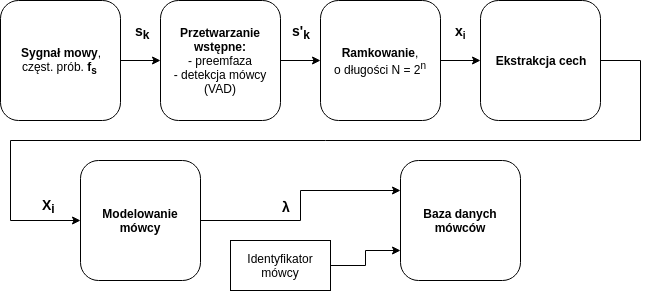
\includegraphics[width=0.9\textwidth]{./fundiagmodel.png}
    \caption{\label{fig:fundiagmodel} Schemat funkcjonalny systemu weryfikacji mówcy dla etapu modelowania.}
\end{figure}

\begin{enumerate}
\item{\textbf{Akwizycja sygnału mowy}} - wejściem całego systemu jest spróbkowany z częstotliowścią $f_s$ sygnał mowy $\bm{s_k}$. Dostarczany jest on z pamięci komputera jako całość lub dostarczany jest w czasie rzeczywistym jako kolejne próbki. Dla tego drugiego przypadku na ten etap składa się realizacja sprzętowa akwizycji sygnału akustycznego mowy za pomocą przetwornika elektroakustycznego oraz przetwornika analogowo-akustycznego. Ważnym elementem jest również odpowiednie filtrowanie
    analogowe sygnału - usunięcie składowej stałej oraz filtrowanie częstotliwości wyższych od połowy częstotliwości próbkowania $f_s$ (filtracja antyaliasingowa).
\item{\textbf{Przetwarzanie wstępne}} - na ten etap mogą składać się wszelkiego rodzaju techniki poprawy jakości sygnału takie jak odszumianie. Najczęściej w systemach weryfikacji mówcy stosuje się tzw. preemfazę - czyli wzmacnianie wyższych częstotliwości sygnału oraz systemy detekcji mówcy (\textit{ang. Voice Activity Detection - VAD})  zwłaszcza dla systemów czasu rzeczywistego. W wyniku przeprowadzonych operacji z sygnału $\bm{s_k}$ otrzymujemy przetworzony sygnał $\bm{s'_k}$.
\item{\textbf{Ramkowanie}} - zwykle w przypadku ekstrakcji cech niskiego poziomu konieczne jest zaaplikowanie ramek na sygnał mowy tak, aby uzyskać chwilowe wektory cech. Dla metod ekstrakcji cech wykorzystujących dyskretne przekształcenie Fouriera (DFT) zwykle dobiera się ramki o długościach równymi $N=2^n$, gdzie n - liczba całkowita. W przypadku takich cech jak LPCC nie jest to warunek konieczny, jednak często stosowany. W wyniku operacji ramkowania otrzymywany jest zbiór wektorów $\bm{x_i}$ o długości N.
\item{\textbf{Ekstrakcja cech}} - na ten etap składa się przetwarzanie ramek sygnału mowy $\bm{x_i}$ na wektory cech oznaczone jako $\bm{X_i}$. Różne techniki wykorzystywane w tym procesie opisano w rozdziale {\ref{featureextraction}}.
\item{\textbf{Modelowanie mówcy}} - w tej części konstruowany jest model mówcy $\bm{\lambda}$ na podstawie zbioru wektorów trenujących $\bm{X_i}$. Różne techniki otrzymywania modeli opisane zostały w rozdziale {\ref{featurematching}}. Model reprezentowany jest najczęściej jako wektor współczynników: w VQ są to centroidy znajdujące się w przestrzeni wektorów, zaś w technice GMM są tą współczynniki wagowe $w_i$ kolejnych funkcji aproksymujących funkcję gęstości prawdopodobieństwa.
\item{\textbf{Zapisanie modelu do bazy danych}} - Wartości parametrów charakteryzujących model mówcy $\bm{\lambda}$ muszą być zapisane na potrzeby fazy weryfikacji. Konieczne jest, aby wraz z modelem została zapisana informacja dotycząca tożsamości mówcy - może być to numer identyfikacyjny w postaci danych charakterystycznych dla mówcy. Identyfikator mówcy jest wykorzystywany w fazie weryfikacji razem z modelem.
\end{enumerate}

\label{pies}

\subsection{Faza weryfikacji.}

Jeżeli system jest w posiadaniu modelu mówcy, za który podaje się mówca, od którego testowany sygnał mowy pochodzi, system weryfikacji mówcy może przeprowadzić procedurę weryfikacji. W tym celu musi przedstawić informację identyfikującą weryfikowanego mówcę. Ogólna struktura procesu weryfikacji mówcy z uwzględnieniem przepływu danych znajduje się na rysunku {\ref{fig:fundiagverif}}. W omawianej procedurze zachowana jest postać algorytmu (rozdział \ref{pies}) aż do momentu uzyskania zbioru wyekstrahowanych cech włącznie. Natomiast zachodzą istotne zmiany co do kolejnych etapów:

\begin{figure}[ht!]
  \centering
    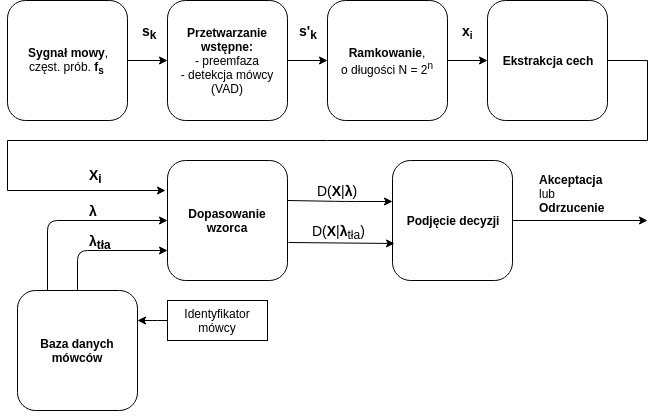
\includegraphics[width=1\textwidth]{./fundiagverif.png}
    \caption{\label{fig:fundiagverif} Schemat funkcjonalny systemu weryfikacji mówcy dla fazy weryfikacji.}
\end{figure}

\begin{enumerate}
    \item{\textbf{Dopasowanie wzorca}} - ten etap korzysta ze zbioru cech $X_i$ w celu weryfikacji mówcy. Podczas tego etapu obliczana jest miara dopasowania pomiędzy wektorami $X_i$ a modelami kolejno $\lambda$ i $\lambda_{tla}$. W tym przypadku model oznaczony jako $\lambda_{tla}$ oznacza albo model tła albo model kohorty (w rozumieniu rozdziału {\ref{verif}}). Wyjściem procesu jest wartość liczbowa tej miary dla obu porównań na rysunku oznaczone jako $D(\bm{X}|\bm{\lambda})$ i $D(\bm{X}|\bm{\lambda}_{tla})$. Dla techniki VQ miara dopasowania to wartość funkcji metryki $d(X,C_n)$ gdzie $C-n$ to centroidy modelu. W przypadku techniki GMM miarą dopasowania jest prawdopodobieństwo.
\item{\textbf{Podjęcie decyzji}} - ostatnim etapem razy weryfikacji mówcy jest podjęcie decyzji. Techniki związane z tym zagadnieniem opisano w rozdziale {\ref{verif}}. Decyzja podejmowana jest na podstawie dwóch liczb dostarczonych z poprzedniego bloku: $D(\bm{X}|\bm{\lambda})$ i $D(\bm{X}|\bm{\lambda}_{tla})$ oraz ustalonego przez projektanta progu $\theta$. Wyjściem całego systemu jest zmienna binarna przyjmująca wartości: Akceptacja lub Odrzucenie.
\end{enumerate}

\section{Architektura systemu weryfikacji mówcy dla czasu rzeczywistego}

Na podstawie przedstawionych schematów funkcjonalnych została zaproponowana architektura oprogramowania dla przetwarzania w czasie rzeczywistym. Ogólny schemat został przedstawiony na rysunku {\ref{fig:overallrt}}. Rozwiązanie oparte jest na użyciu trzech bloków przetwarzania oraz trzech buforów typu fifo (\textit{ang. first in firts out}). Projekt oparty jest na podejściu producent-konsument, tzn. występuje blok produkujący dane przekazywane do kolejki FIFO - nazwany producentem oraz blok
odbierający dane z kolejki FIFO - nazwany konsumentem.  W omawianym rozwiązaniu zawsze występuje tylko jeden producent i jeden konsument. Takie bloki mogą zostać zaimplementowane w zwykłym systemie operacyjnym jako wątki, w systemie czasu rzeczywistego jako 'taski' oraz sekwencyjnie w przypadku braku takiego wsparcia ze strony systemu uruchomieniowego. 

\begin{figure}[ht!]
  \centering
    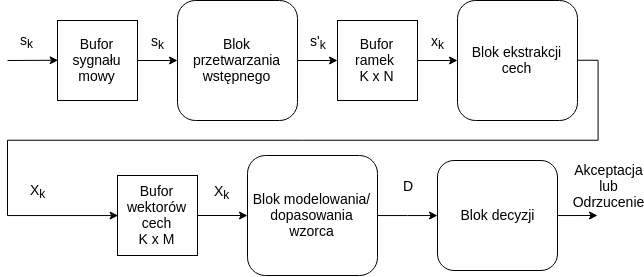
\includegraphics[width=1\textwidth]{./overallrt.png}
    \caption{\label{fig:overallrt} Schemat funkcjonalny architektury systemu weryfikacji dla przetwarzania w czasie rzeczywistym.}
\end{figure}

\subsection{Bufory FIFO}

Głównym zadaniem użytego w systemie buforu typu FIFO (kolejki) jest kontrola przepływu danych. Stan przepełnienia lub wyczerpania kolejki stanowi podstawę do sterowania kontekstem wykonywanego zadania. W systemie występują trzy kolejki przystosowane do różnego typu danych:
\begin{itemize}
\item{\textbf{Bufor sygnału mowy}} - jest to bufor FIFO przechowujący kolejne, nadchodzące próbki sygnału mowy. Może być zrealizowany programowo - dodatkowy wątek lub blok programu odpowiedzialny jest za jej napełnianie poprzez wywołanie odpowiednich wywołań systemowych lub za pomocą przerwania. Blok przetwarzania wstępnego jest w tym przypadku konsumentem i odbiera kolejne próbki z kolejki.
\item{\textbf{Bufor ramek}} - jest to bufor FIFO przechowujący kolejne ramki sygnału o stałym rozmiarze $N$. Ramki produkowane są przez blok przetwarzania wstępnego i wysyłane do tejże struktury danych. Odbiorcą jest blok ekstrakcji cech.
\item{\textbf{Bufor wektorów cech}} - jest podobny do buforu ramek, różni się jedynie mniejszym rozmiarem ramki dla wektora cech o długości $M$. 
\end{itemize}

\subsubsection{Implementacja kolejki FIFO}

Kolejki różnią się implementacją w zależności od wybranego systemu uruchomieniowego:
\begin{itemize}
\item{\textbf{System czasu rzeczywistego - RTOS}} - w tego typu systemach znajdują się gotowe implementacje kolejek przystosowane do synchronizacji pomiędzy taskami. Przykładem takiej struktury jest \textit{xQueue} w systemie operacyjnym \textit{FreeRTOS} \cite{freertos}.
\item{\textbf{Wielowątkowy system operacyjny}} - ponieważ w bibliotece standardowej nie znajdują się struktury danych umożliwiające bezpieczną pracę w środowisku wielowątkowym potrzebna jest inna implementacja kolejki niż standardowa \textit{stdqueue}. Implementacja może pochodzić z zewnętrznej biblioteki takiej jak \textit{boost} albo \textit{QT}. Jednak łatwo jest zaimplementować omawianą strukturę danych przy pomocy algorytmu wzajemnego wykluczenia (\textit{ang. mutex}) znajdującego się w
    bibliotece standardowej pod nazwą - \textit{std::mutex}. Poniżej podano przykładową implementację, z której korzysta się w przykładowym systemie opisanym w niniejszej pracy.
\begin{lstlisting}[style=lst:cpp, caption=Bezpieczna wątkowo kolejka\label{lst:queue}]
template <class T>
class queue
{
  public:
  ...
    T pop()
    {
      //zajecie mutexu
      std::unique_lock<std::mutex> mutex_lock(mutex_);
      while(queue_.empty()) // zablokuj watek jesli pusta
      {
        condition_.wait(mutex_lock);
      }
      auto item = queue_.front(); // pobierz element
      queue_.pop(); //usun obiekt z kolejki
      return item;
    }

    void push(T&& object)
    {
      //zajecie mutexu
      std::unique_lock<std::mutex> mutex_lock(mutex_);
      queue_.push(std::move(item)); // dodaj obiekt na koniec kolejki
      mutex_lock.unlock(); // zwolnij mutex
      condition_.notify_one(); // zaktualizuj zmienna condition_
    }
  ...

  private:
    std::queue<T> queue_;
    mutable std::mutex mutex_;
    std::condition_variable condition_;
};
\end{lstlisting}

Dla podanej implementacji zachowano podobną semantykę wezwań, tak jak w przypadku kolejki \textit{std::queue}: funkcja \textit{pop()} zwraca pierwszy element kolejki, zaś funkcja \textit{push()} umieszcza obiekt na końcu kolejki. Aby zapobiec zjawisku wyścigu użyta została blokada \textit{std::mutex} podczas odczytu i zapisu z kolejki. Z kolei obiekt \textit{std::condition\_variable} z biblioteki standardowej realizuje blokadę wątku odczytującego w przypadku, kiedy kolejka jest pusta. Wywołanie
        w linii 25 informuje zablokowany wątek o uzupełnieniu kolejki o jeden element. Pętla w linii 10 zapobiega zwolnieniu wątku w przypadku, gdy wystąpi inny powód odblokowania wątku niż powiększenie się kolejki.


\item{\textbf{Brak systemu uruchomieniowego}} - w przypadku braku środowiska wielowątkowego nie jest potrzebne zapewnienie kontenera bezpiecznego wątkowo (\textit{ang. thread safe}). Dlatego wystarczy wykorzystać gotową strukturę kolejki z biblioteki standardowej \textit{std::queue}.
\end{itemize}

\subsubsection{Kolejność wykonywania bloków}

W przypadku korzystania ze wsparcia systemu operacyjnego sprawa jest najprostsza - kolejne bloki implementowane są jako niezależne wątki synchronizowane za pomocą kolejek. Jeżeli jednak system nie korzysta ze wsparcia środowiska uruchomieniowego potrzebna jest implementacja odpowiedniej logiki sterującej. Na rysunku {\ref{fig:logics}} przedstawiono propozycję algorytmu sterowania wykonaniem w tego typu systemie.

\begin{figure}[ht!]
  \centering
    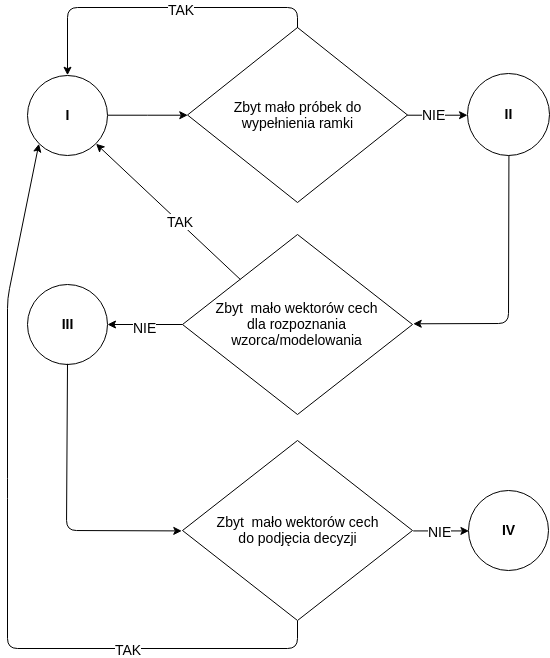
\includegraphics[width=0.6\textwidth]{./logic.png}
    \caption{\label{fig:logics} Algorytm sterownia bez wsparcia systemu operacyjnego. \textbf{Blok I} - blok wstępnego przetwarzania. \textbf{Blok II} - blok ekstrakcji cech. \textbf{Blok III} - blok rozpoznania wzorca/modelowania. \textbf{Blok IV} - blok podejmowania decyzji.}
\end{figure}

\subsection{Bloki przetwarzania}
Poniżej opisano trzy bloki przetwarzania znajdujące się w systemie. Bloki realizują funkcjonalności, które opisano w {\ref{funcioniert}}.
\begin{itemize}
\item{\textbf{Blok wstępnego przetwarzania}} - realizuje funkcjonalności przetwarzania wstępnego oraz ramkowania z rysunku {\ref{fig:fundiagverif}}. Wszystkie wykorzystywane funkcje w tym bloku zdefiniowane są w przestrzeni nazw \textit{dsp\_utils}. 
\item{\textbf{Blok ekstrakcji cech\label{archfeatureextraction}}} - realizuje funkcjonalność ekstrakcji cech. 
\item{\textbf{Blok rozpoznawania wzorca/modelowania\label{archpatternmatching}}} - realizuje funkcjonalność dopasowania wzorca oraz modelowania.
\item{\textbf{Blok podejmownia decyzji}} - realizuje funkcjonalność podejmowania decyzji o weryfikacji.
\end{itemize}


\subsection{Baza danych mówców}
Dany mówca reprezentowana jest jako następująca struktura danych dla systemu weryfikacji mówcy z wyświetlanym hasłem:
\begin{lstlisting}[style=lst:cpp, caption=struktura danych przechowująca informację o mówcy\label{lst:database}]
template <int C, int K>
using codebook_array = typename std::array<std::array<double, K>, C>; 


class speaker {
  public:
    speaker(const std::string& name)
      : speaker_info{name} {}  

    std::string name() {return speaker_info.name;};

    struct Code{
      Code(const std::string& text, codebook_array<C,K>&& code)
        : centroids{code}, text{text} {}
      std::array<std::array<double, K>, C> centroids;
      std::string text;
    };

    void add_code(speaker::Code&& code)
    {
      codebook.push_back(code); 
    }

  private:
    std::vector<Code> codebook;

    struct speaker_info{
      speaker_info(const std::string& name)
        : name{name} {}
      std::string name;
    } speaker_info;
};
\end{lstlisting}

Klasa \textit{speaker} zawiera dwie struktury danych: instancję struktury \textit{speaker\_info}, która reprezentuje numer identyfikacyjny mówcy przy pomocy zmiennej łańcuchowej \textit{name} oraz instancji struktury \textit{codebook} przechowującej wektory współczynników charakteryzujących modele (w przypadku metody VQ są to centroidy - stąd nazwa zmiennej \textit{centroids}). Alias do tablicy dwuwymiarowej, z której korzysta implementacja to \textit{codebook\_array}.
